%---Packages---%
\documentclass[a4paper,11pt]{article}
\usepackage[left=2.5cm,top=2cm,right=2cm,nohead]{geometry}
\usepackage[french]{babel}
\usepackage[T1]{fontenc}
\usepackage[utf8]{inputenc} 
\usepackage{graphicx}
\usepackage{float}
\usepackage{amsmath}
\usepackage{amsfonts}
\usepackage{amssymb}
\usepackage{listings}
\usepackage{mdwlist}
\usepackage[usenames,dvipsnames]{color}
\usepackage[stable]{footmisc}%To include footnotes in 'section' parts
\usepackage{hyperref}
\usepackage{setspace}
\usepackage{eurosym}
\usepackage[section]{algorithm} % [section] is use to define the numbering mode
\usepackage{algorithmic} 

%---Insertion de code---%
\definecolor{lightgray}{gray}{0.95}


\lstset
{           
backgroundcolor=\color{lightgray},
keywordstyle=\color{Red}\bfseries,
ndkeywordstyle=\color{darkgray}\bfseries,
commentstyle=\color{Green},
stringstyle=\color{Orange},
basicstyle=\footnotesize,       % the size of the fonts that are used for the code
numbers=left,                   % where to put the line-numbers
numberstyle=\footnotesize,      % the size of the fonts that are used for the line-numbers
stepnumber=2,                   % the step between two line-numbers. If it's 1 each line will be numbered 
numbersep=5pt,                  % how far the line-numbers are from the code
showspaces=false,               % show spaces adding particular underscores
showstringspaces=false,         % underline spaces within strings
showtabs=false,                 % show tabs within strings adding particular underscores
tabsize=2,	                % sets default tabsize to 2 spaces
captionpos=b,                   % sets the caption-position to bottom
breaklines=true,                % sets automatic line breaking
breakatwhitespace=false,        % sets if automatic breaks should only happen at whitespace
title=\lstname,                 % show the filename of files included with \lstinputlisting & 
escapeinside={\%*}{*)},         % if you want to add a comment within your code
morekeywords={*,...}            % if you want to add more keywords to the set
extendedchars=true
}

%---Liens---%
\hypersetup{
unicode=false,          % non-Latin characters in Acrobat’s bookmarks
pdftoolbar=true,        % show Acrobat’s toolbar?
pdfmenubar=true,        % show Acrobat’s menu?
pdffitwindow=false,     % window fit to page when opened
pdfstartview={FitH},    % fits the width of the page to the window
pdftitle={Projet AGGP - Synthèse des articles},    % title
pdfauthor={Balthazar Rouberol, Anthony Tschirhard, Marion Poirel, Marie Paturel},     % author
pdfsubject={Projet AGGP - Dossier d'init},   % subject of the document
pdfcreator={Balthazar Rouberol, Anthony Tschirhard, Marion Poirel, Marie Paturel},   % creator of the document
pdfkeywords={Réseaux biologiques, Réseaux, AlgoGen}, % list of keywords
pdfnewwindow=true,      % links in new window
colorlinks=true,       % false: boxed links; true: colored links
linkcolor=black,          % color of internal links
citecolor=black,        % color of links to bibliography
filecolor=white,      % color of file links
urlcolor= NavyBlue,           % color of external links
bookmarks=true,% show bookmarks bar?
bookmarksopen=false,
bookmarksnumbered = false      
}%



\begin{document}
\maketitle

L'objectif de ce document est de prévoir la conception du projet en explicitant l'organisation du code ainsi que le planning des phases de codage, de tests et d'exploitation du code. Ainsi, sa lecture devrait permettre de connaître précisément la division du projet, à la fois au niveau humain (organisation au sein de l'équipe) et temporel.

%%%%%%%%%%%%%%%%%%%%%%%%%%%%%%%%%%%%%%%%%
\section{Présentation générale du projet}

\subsection{Algorithme génétique}
Le but de ce projet est de faire évoluer une population de réseaux grâce à un algorithme génétique pré-existant. Nous devons définir une \textit{fitness} qui permet de sélectionner les individus sur leurs capacités à s'approcher d'un réseau biologique.

Un individu correspondant à un réseau, le génome manipulé par l'algorithme génétique est une concaténation des lignes de la partie triangulaire supérieure de la matrice d'adjacence du réseau. Celle-ci étant ici symétrique, le réseau est ainsi parfaitement représenté.

\subsection{Livrables et délais}

\subsection{L'équipe}
\begin{itemize}
\item Chef de Projet : Balthazar Rouberol
\item Responsable Qualité : Marion Poirel
\item Ma\^itre d'œuvre : Anthony Tschirhard
\item Responsable Documentation : Marie Paturel
\item Groupe d'étude informatique : Balthazar Rouberol, Anthony Tschirhard, Marion Poirel, Marie Paturel
\end{itemize}



%%%%%%%%%%%%%%%%%%%%%%%%%%%%%%%%%%%%%%%%%%%%%%%%%%%%%%%%%%
\section{Rappel sur les réseaux biologiques}
% Anthony
Afin d'être le plus proche possible d'un réseau biologie, il convient de connaitre ses caractéristiques et paramètres associés. Les réseaux que nous allons créer et faire évoluer vont devoir répondre à trois grandes caractéristiques : la répartition de ses degrés devra suivre une \textit{loi exponentielle}, il devra vérifier la propriété dite de \textit{\og petit monde \fg} et devra contenir des \textit{cliques}.

\subsection{Répartition des degrés -- Loi exponentielle}
% Anthony
\begin{wrapfigure}{r}{0.5\textwidth}
  \vspace{-30pt}
  \begin{center}
    \includegraphics[width=0.50\textwidth]{plot.png}
  \end{center}
  \caption{Réseau dont la distribution suit une loi exponentielle}
  \label{scalefree}
\end{wrapfigure}
La répartition des degrés d'un réseau dit \textit{scale-free} suit une loi exponentielle. Comme le montre la figure~\ref{scalefree}, les degrés des nœuds d'un réseau diminuent quand leur nombre augmente. Autrement dit, on va avoir très peu de nœuds très fortement connectés et beaucoup de nœuds fortement connectés. La loi que suit cette répartition de degrés est la suivante :
$$ P(k) ~ \alpha k^{-g} $$

On a donc des nœuds très connectés appelés \textit{\textbf{hubs}} et une très grande majorité de nœuds très faiblement connectés.	Les articles étudiés dans le cadre de ce projet nous informent que $g$ doit être compris entre $2$ et $3$, et de manière plus précise entre $2.1$ et $2.3$. Nous avons donc décidé de prendre arbitrairement la valeur de $g=2.2$\footnote{todo : référence à l'article en question !}. Nous allons donc partir de ces deux hypothèses pour implémenter la fonction de répartition des degrés qui entrera en compte dans la détermination de la fonction de \textit{fitness}.

Afin de faire cela, nous allons donc parcourir l'ensemble des nœuds du graphe et calculer la fréquence de chaque degré. Ensuite, nous comparerons la répartition obtenue à la loi de puissance "optimale" -- dans la cadre de notre modèle. Afin de déterminer l'écart à cette loi, nous calculerons le carré de la distance entre la valeur réelle et la valeur de référence.

\subsection{Propriété de petit monde}
% Anthony
La propriété de \textbf{petit monde} nous indique que deux nœuds du réseau biologique sont reliés en moyenne par une distance $n$ optimale. Dans ce projet, et considérant le réseau biologique étudié (todo), nous avons décidé de prendre une valeur de $n=...$.

Afin d'avoir accès à cette valeur moyenne, nous nous servirons une fonction du package \verb?NetworkX? qui nous fournira directement ladite valeur. Nous la comparerons ensuite à la valeur théorique\footnote{On dit que dans un réseau social, deux individus pris au hasard sur Terre sont connectés entre eux par l'intermédiaire de $6$~personnes.}.

\subsection{Formation de cliques -- coefficient de \textit{clustering}}
% Anthony
Un graphe compte un certain nombre de \textbf{cliques} de différentes tailles. Une clique est un ensemble de nœuds entièrement interconnectés. Le \textbf{coefficient de clustering} est un bon indicateur de la présence de cliques et se calcule pour chaque nœud de la manière suivante :
$$ C_i = \frac{2Ei}{k_i k_{i-1}} $$
avec
\begin{itemize}
 \item $E_i$ : nombre de liens entre voisins ;
 \item $k_i$ : nombre de voisins de $i$.
\end{itemize}
Nous allons utiliser le coefficient de \textit{clustering} global, c'est à dire la moyenne des coefficients de chaque nœud. Ainsi, nous aurons une valeur comprise entre $0$ et $1$ que nous pourrons utiliser dans notre fonction de \textit{fitness}.


%%%%%%%%%%%%%%%%%%%%%%%%
\section{Implémentation}
% Anthony

\subsection{Classes et objets}
% Anthony
\begin{figure}
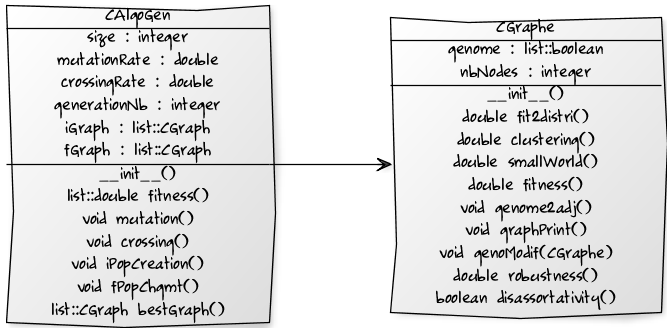
\includegraphics[width=\linewidth]{diagramme}
\caption{Diagramme de classe}
\label{diag}
\end{figure}
Comme le montre la figure~\ref{diag}, 

\subsection{Codage d'un réseau}
% Anthony
\subsubsection{Matrice d'adjacence}
\subsubsection{Remplissage de la matrice}
\subsubsection{Fonctions}

\subsection{Algorithme génétique}
%Afin de minimiser le temps de convergence, nous partons d'une distribution biaisée : la matrice est remplie selon une loi de puissance.
%
%On considère qu'un réseau est biologique s'il possède les trois propriétés suivantes :
%\begin{itemize}
%\item distribution des degrés selon une loi exponentielle de paramètre $2.2$\footnote{article ?} ,
%\item "petit monde",
%\item présence de cliques.
%\end{itemize} 
%
%A chaque génération, on vérifie l'adéquation de chaque réseau avec ses caractéristiques : leur somme pondérée définit la \textit{fitness} d'un individu. Les individus sont classés en fonction de leur \textit{fitness} et sélectionnés selon le procédure suivante : ???. Ceux conservés pour la nouvelle génération subissent des mutations, des \textit{crossing-over} (et des croisements ?), étapes fondamentales de l'évolution.
%
%Une fois la génération finale obtenue, on teste la robustesse des réseaux (conservation des propriétés malgré la suppression au hasard d'un nœud) ainsi que leur concordance avec la disassortativité (les hubs ne sont pas reliés entre eux).\\
%
%Cette simulation est faite plusieurs fois, sur X pas de temps (temps moyen de convergence, explication ?). Les paramètres finaux des réseaux sont conservés afin de permettre un étude comparative. D'un simulation à une autre, la pondération des paramètres de la loi de \textit{fitness} et le degré de la loi de puissance pourront varier, ce qui permet d'étudier leur impact respectif.

\subsection{Fonction de \textit{fitness} }
%Combinaison libéaire de fonction
%Pourquoi pondérer ?

%%%%%%%%%%%%%%%%%%%%%%%%%%%%%%%%%%%%%%%%%
\section{Planning}
\subsection{Répartition du code}

\subsection{Phases de tests}

\subsection{Exploitation}

\subsection{Risques}


\end{document}